%%%%%%%%%%%%%%%%%%%%%%%%%%%%%%%%%%%%%%%%%%%%%%%%%%%%%%%%%%%%%%%%%%%%%%%%
% Plantilla TFG/TFM
% Escuela Politécnica Superior de la Universidad de Alicante
% Realizado por: Jose Manuel Requena Plens
% Contacto: info@jmrplens.com / Telegram:@jmrplens
%%%%%%%%%%%%%%%%%%%%%%%%%%%%%%%%%%%%%%%%%%%%%%%%%%%%%%%%%%%%%%%%%%%%%%%%

\chapter{Introducción}

\section{Motivación y contexto}
\bibliographystyle{apacite}

Mi interés por la visión artificial se desarrolló durante el tercer año de carrera, donde me presenté junto a la Universidad de Alicante a un proyecto llamado Vodafone Campus Lab[\cite{Vodafone}], donde te proponen unos problemas a resolver y nosotros decidimos plantear una solución con tecnologías como la visión artificial. Además esta propuesta requería de procesos como la adquisición del cuerpo 3D y reconocimiento de este, entre otros. Aquí fue cuando busqué propuestas de trabajo final de grado (TFG) similares o sobre este tema porque me quedé con la curiosidad de llevarlo a cabo y porque quería saber, aprender e investigar más sobre la adquisición de modelos 3D a partir de imágenes, cuando vi las propuestas fue cuando conocí el proyecto de investigación [\cite{tech}].

El proyecto de investigación Tech4Diet cuenta con el apoyo de la Agencia Estatal de Investigación (AEI) y del Fondo Europeo de Desarrollo Regional (FEDER) con referencia "TIN2017-89069-R" perteneciente al programa Retos 2017 en el que su investigador jefe es Jorge Azorín. En este proyecto se busca facilitar el estudio de la evolución morfológica ocasionada por tratamientos de obesidad. Hoy en día, estos tratamientos son muy costosos pero a su vez muy necesarios, ya que los problemas de obesidad o sobrepeso pueden ocasionar enfermedades crónicas como la hipertensión, diabetes tipo II, cáncer. También pueden ocasionar enfermedades patológicas neurodegenerativas como el Alzheimer o demencias [\cite{Andres1}]


El sistema utilizado para esta finalidad, dispone de una red de cámaras RGB-D que
obtienen un modelo 3D del cuerpo del paciente. El proceso de obtención de un modelo 3D se realiza en diferentes sesiones médicas, lo que permite una visualización real de la evolución del cuerpo del paciente. Para que el paciente pueda visualizar su progreso, no solo dispondrá de una aplicación de ordenador, sino que también podrá visualizar los diferentes modelos de su cuerpo mediante unas gafas de realidad virtual. La realidad virtual tiene como finalidad incrementar la adherencia del usuario al tratamiento. Además, podemos encontrar desarrollos tecnológicos como "Google Cardboard" que nos permiten convertir cualquier teléfono móvil en unas gafas de realidad virtual sin necesidad de realizar un gasto de dinero elevado.
A parte de la visualización, sobre este modelo 3D obtenido con las cámaras se pueden realizar mediciones de diferentes partes del cuerpo a niveles de 1D, 2D y 3D. 

\begin{figure}[H]
	\centering
	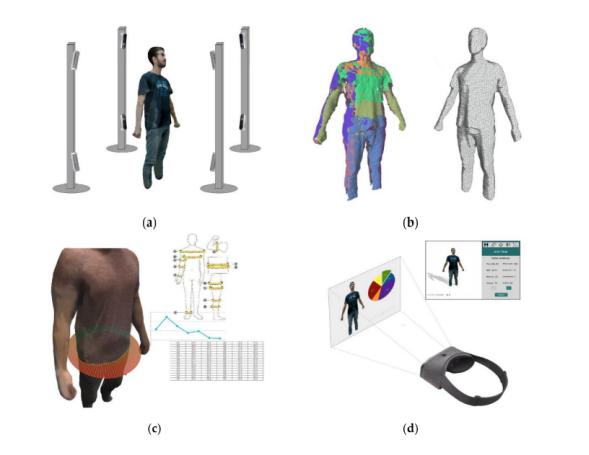
\includegraphics[scale=0.7]{imagenes/intro1.png}
	\caption{Captación del modelo del cuerpo mediante el sistema de cámaras (a). Nubes de puntos sin textura generada (b). Mediciones del cuerpo (c). Visualización de los resultados en la aplicación y con gafas de realidad virtual [\cite{Nahuel1}]}
	\label{fig:figura1}
\end{figure}

En este contexto, este trabajo final de grado tiene como objetivo principal la reconstrucción de modelos 3D del cuerpo humano con textura, a partir de imágenes 2D  adquiridas con dispositivos de consumo como las disponibles en teléfonos móviles. Esto permite mejorar la portabilidad y coste de sistemas basados en redes de cámaras RGBD, como es el caso de Tech4diet[\cite{tech}]. En este TFG se analizará de forma comparativa la precisión de las medidas de los modelos 3D obtenidos en relación a las medidas obtenidas mediante los sistemas más costosos como el de Tech4diet.

\newpage
\section{Objetivos}


%\par Esto es una cita estándar: \citet{Shaw1996}, que también puedes mostrar con paréntesis así: \citep{Shaw1996}. También se puede realizar una cita indicando a qué parte te refieres \citep[ver][Cap. 2]{Shaw1996} o \citep[Cap. 2]{Shaw1996} o \citep[ver][]{Shaw1996}. 

%\par También puedes mostrar todos los autores cuando hay más de 2 autores añadiendo un asterisco después del comando como: \citet*{Akyildiz2005}, sin el asterisco quedaría así: \citet{Akyildiz2005}.

%\par O puedes citar dos o más fuentes al mismo tiempo: \citep{Barkan1995,Leighton2012}

Como se ha mencionado, el objetivo general del trabajo fin de grado es la reconstrucción de modelos 3D del cuerpo humano con textura, a partir de imágenes 2D adquiridas con dispositivos de consumo, como las disponibles en teléfonos móviles. Para alcanzar este objetivo general se plantean los siguientes específicos:


\begin{itemize}
	\item{\textbf{Objetivo 1: Analizar métodos del estado del arte para la reconstrucción del modelo 3D del cuerpo humano a partir de imágenes 2D.}} 
	
	\item{\textbf{Objetivo 2: Análisis y adaptación del modelo PIFu[\cite{pifu}] para la obtención de modelos 3D con textura a partir de vistas 2D del cuerpo humano  }} \\
	Para este objetivo se tendrán que realizar las siguientes tareas específicas:
	\begin{itemize}
		\item Estudio de los diferentes parámetros para el entrenamiento y prueba de la red propuesta en PIFu.
		\item Obtención de imagen del cuerpo y generación de máscara de la imagen.
		\item Obtención y estudio de los resultados.
		
	\end{itemize}
	
	\item{\textbf{Objetivo 3: Análisis comparativo de la precisión de las medidas obtenidas a partir de modelos 3D del cuerpo humano }} \\
	\begin{itemize}
		\item Estudio sobre las diferentes formas de realizar el cálculo de las diferencias obtenidas.
		\item Alineamiento de objetos 3D.
		\item Cálculo de distancias usando Hausdorff Distance
		\item Cálculo de distancias usando Chamfer distance
	\end{itemize}
\end{itemize}
\clearpage

\section{Estado del arte}
%\begin{verbatim}
La reconstrucción del cuerpo humano 3D es un tema amplio abordado de diferentes maneras. Por una parte tenemos la visión por computador que nos permite entender la información visual del entorno capturada a través de las cámaras [\cite{Zhang1}]. Por otra parte nos encontramos avances recientes en la estimación del cuerpo humano 3D basado en imágenes que han sido impulsados por la mejora significativa en el poder de representación que ofrecen las redes neuronales profundas. [\cite{pifuhd}]

Se ha llevado a cabo una revisión del estado del arte que abordan las diferentes formas de obtener resultados respecto a la reconstrucción del cuerpo humano.
\\

Recientes trabajos abordados mediante el uso de la visión por computador utilizan cámaras RGB-D calibradas [\cite{Nahuel1}]. El trabajo abordado por García D'Urso propone el uso de dispositivos RGB-D (como Microsoft Kinect o Intel RealSense), debido a que integran sensores de color y profundidad, y utilizan tecnologías de profundidad como luz estructurada, ToF (Time of Flight, sensor que mide distancias utilizando el tiempo que usan los fotones en viajar entre dos puntos) o activa estereoscópica. En este proyecto aparte de la obtención del modelo, también se han tratado otros puntos como la visualización 3D del cuerpo utilizando la realidad virtual, además de que pueden obtener las medidas de volúmenes seleccionados del cuerpo humano. Con esta propuesta llevan a cabo una red de cámaras RGB-D formado por 13 cámaras ubicadas en una cabina donde la persona se ha de colocar durante 4 segundos como se puede ver en la figura \ref{fig:figura2}. Esta red de cámaras se ha de calibrar de manera que cada una de ellas quede calibrada intrínsicamente y extrínsecamente para cada cámara y multi-cámara para así estimar la posición relativa de cada sensor en la red, una vez la red de cámaras se encuentren calibradas sigue el proceso de la obtención del modelo 3D con textura que consta de 5 fases principales, que se ven en la figura \ref{fig:figura1}: adquisición, pre-procesado, unión de vistas, generación de la malla y proyección de la textura.
\begin{figure}[H]
	\centering
	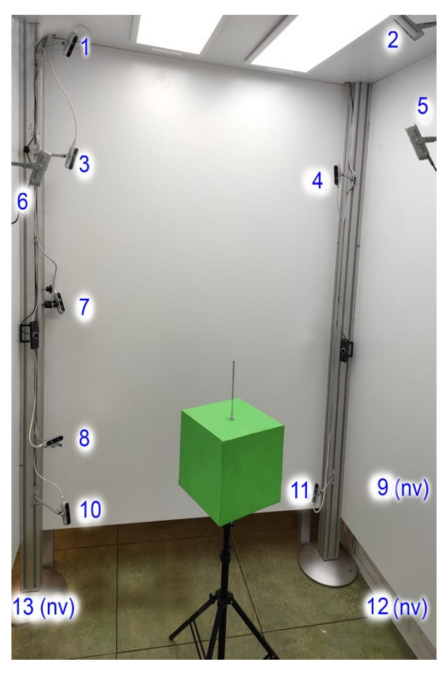
\includegraphics[scale=0.35]{imagenes/estadoarte1.png}
	\caption{Set-up de red de 13 cámaras RGB-D. "nv" indica que la cámara no está visible en la imagen [\cite{Nahuel1}].}
	\label{fig:figura2}
\end{figure}


Actualmente, nos encontramos recientes trabajos abordados mediante el uso de visión artificial y deep learning, en estos a diferencia del anterior no se necesita una cabina formada por una red de cámaras. Todos estos trabajos tienen el mismo objetivo: producir resultados naturales y bien alineados [\cite{pymaf}], en concreto han habido varios paradigmas investigados, desde una visión basada en la optimización que ajusta explícitamente los modelos a las imágenes 2D [\cite{keepsmpl}], dentro de este paradigma nos encontramos con el trabajo de investigación por parte de Bogo que desarrolla un método para automáticamente estimar la pose y forma 3D del cuerpo humano a partir de una imagen, para ello siguen dos pasos, primero estiman los 2D joints (uniones, en este caso sería por ejemplo la rodilla que une la parte inferior y superior de la pierna), esto lo consiguen usando una red neuronal convolucional (CNN) llamado DeepCut [\cite{deepcut}]. Esta red es buena estimando la pose 2D pero no bueno con la pose 3D por lo que el siguiente paso es el que estima la pose y la forma 3D partiendo de los 2D joints utilizando el modelo SMPL [\cite{smpl}] ajustando dentro de un paradigma clásico bottom up de estimación (CNN) seguida de una verificación descendente (modelo generativo), como se puede ver en la figura \ref{fig:figura3}:
\begin{figure}[!h]
	\centering
	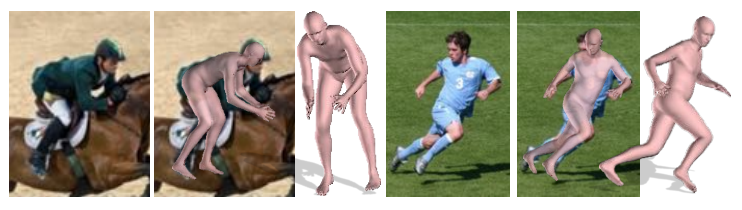
\includegraphics[scale=0.7]{imagenes/estadoarte2.png}
	\caption{Ejemplos. forma y pose 3D estimada mediante el método desarrollado por Bogo[\cite{keepsmpl}] usando las fotos de Leeds Sports Pose Dataset[\cite{edafig2}]. Se ve la imagen original a la izquierda, luego el modelo comparado en la foto en el centro y por último a la derecha el modelo 3D desde otro punto de vista. }
	\label{fig:figura3}
\end{figure}
\\
Los métodos basados en la optimización como el de Bogo ajustan explícitamente los modelos a las imágenes, lo que produce resultados con buena precisión de los alineamientos entre malla-imagen, pero tienden a ser lentos y sensibles al inicio[\cite{pymaf}].

En cambio, desde el enfoque de los modelos basados en regresión nos sugieren directamente predecir el modelo a partir de los parámetros de las imágenes [\cite{pymaf}]. En este apartado nos encontramos propuestas similares a la de H. Zhang, estos modelos se basan en los parámetros existentes en las imágenes y están demostrando resultados prometedores pero aún existen errores principalmente de alineamientos entre malla e imagen, para resolver este problema H. Zhang  propone y diseña PyMAF (Pyramidal Mesh Alignment Feedback). 

La idea central de este enfoque es corregir las desviaciones paramétricas de manera explícita y progresiva basado en el estado del alineamiento, en PyMAF el alineamiento se realiza extrayendo las características espaciales respecto a la proyección 2D de la malla estimada y luego retroalimenta los regresores para que actualicen los parámetros.
\begin{figure}[H]
	\centering
	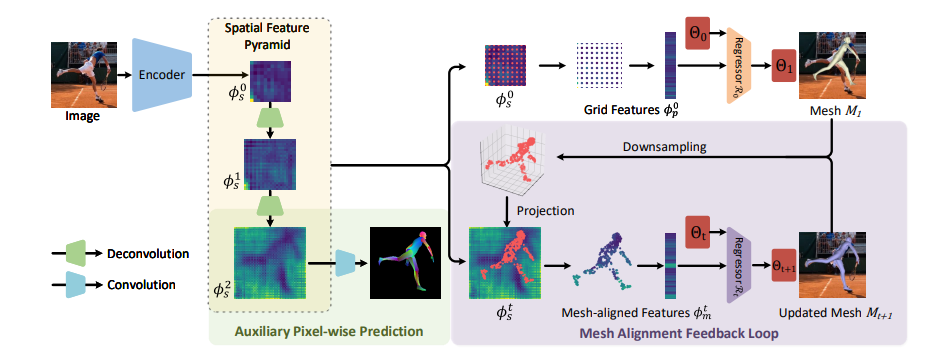
\includegraphics[scale=0.6]{imagenes/estadoarte3.png}
	\caption{ Descripción general de la propuesta PyMAF. PyMAF aprovecha una Feature Pyramid. Dada una predicción del modelo, los alineamientos de la malla son extraídos de características de una resolución más fina y retroalimentan el regresor para así actualizar la malla.  [\cite{pymaf}]   }
	\label{fig:figura4}
\end{figure}

Existe otro tipo de paradigma investigado que esta basado en la representación por vóxeles [\cite{Voxel}] (un vóxel representa un valor en una malla de tres dimensiones) en este nos encontramos con el proyecto conocido como BodyNet [\cite{bodynet}]. Varol propone una red neuronal entrenable de extremo a extremo enfocada en la inferencia directa de la forma volumétrica del cuerpo a partir de una sola imagen. Esta red genera probabilidades en el campo de ocupación 3D de la malla de una persona, dado que se usa una sola vista hay existen pérdidas de información que tratan de solventar aproximando el espacio de vóxeles, aumentando la importancia de los vóxeles que se encuentran en la frontera del cuerpo de la persona y el resto de imagen.

\begin{figure}[!h]
	\centering
	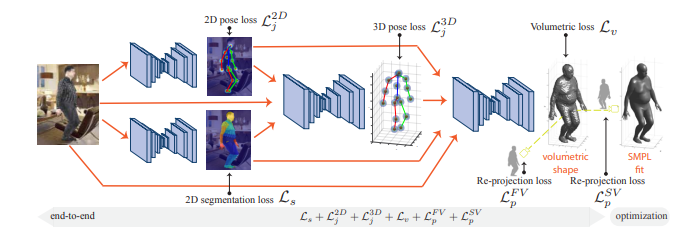
\includegraphics[scale=0.6]{imagenes/estadoarte4.png}
	\caption{ Arquitectura general de la propuesta BodyNet[\cite{bodynet}]. Donde comienza a partir de una imagen RGB que se le pasa a dos subredes donde estiman tanto la pose como la segmentación 2D, con estas predicciones y la imagen se utilizan como  entrada para la siguiente red, que estima en este caso la pose 3D, con todo lo anterior se utiliza como entrada en la siguiente red donde obtiene ya la forma del cuerpo, donde ya por último se ajusta con el modelo SMPL[\cite{smpl}]}
	\label{fig:figura5}
\end{figure}

Al mismo tiempo, hay proyectos como el que se explicará detalladamente en los siguientes puntos como PIFu[\cite{pifu}] que consta de una función que alinea localmente píxeles de imágenes 2D con el contexto global de su objeto 3D correspondiente, para ello se propuso el uso de una red neuronal profundo de extremo a extremo la cual es capaz de representar a humanos de manera que tanto el pelo como la ropa se ve detallada, que es uno de los puntos débiles de los proyectos mencionados con anterioridad, dado que estos [\cite{keepsmpl},\cite{pymaf}] realmente no representan la ropa ni el pelo, tan solo la pose y el cuerpo es una representación del cuerpo humano desnudo, a diferencia de el proyecto llevado a cabo po Fuster-Guilló [\cite{Andres1}, \cite{Nahuel1}], este proyecto si que es capaz de representar la ropa.

Además de la reconstrucción del cuerpo 3D, existe otro punto esencial que es la obtención de la textura del modelo 3D, por este lado podemos observar que mientras realiza PIFu[\cite{pifu}] una estimación directa de los colores RGB mediante una función implícita, también existen más maneras de representar la textura como la parametrización de la superficie como por ejemplo [\cite{texture1}, \cite{densepose}] al igual que en el PIFu[\cite{pifu}] que aparte de la representación de la textura en un objeto 3D, representan dicho objeto 3D, Kanazawa propone 
\begin{figure}[!h]
	\centering
	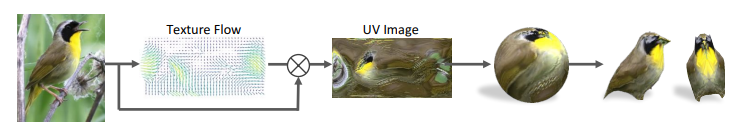
\includegraphics[scale=0.6]{imagenes/estadoarte5.png}
	\caption{Ciclo de obtención de textura[\cite{texture1}]}
	\label{fig:figura6}
\end{figure}

Como podemos ver en la figura \ref{fig:figura6}, se predice el flujo de textura $F$ que es usado como  entrada a la vez que la propia imagen inicial $I$ para generar la imagen de la textura $I^{uv}$ esta imagen es a su vez utilizada para texturizar la malla obtenida en la reconstrucción del modelo 3D.


Güler en su propuesta reconstruye una malla del cuerpo humano, una vez la tiene segmenta esta malla en diferentes partes, de esta malla obtienen las coordenada que luego son utilizadas para renderizar un píxel de manera que se compara directamente la posición verdadera y luego mapean directamente una textura RGB que han utilizado de [\cite{Varol_2017}] a las coordenadas corporales UV estimadas.


Con esta investigación del estado del arte podemos observar que hay diferentes maneras de realizar la reconstrucción del cuerpo humano, dentro de cada manera hay varios trabajos parecidos dado que unos se retroalimentan de otros, también hemos visto de que manera obtienen la textura este tipo de métodos donde a partir de una imagen reconstruyen un modelo 3D. 

En general, os trabajos realizados mediante visión artificial y redes neuronales están más enfocados en general a las poses de las personas, dado que comenzó inicialmente en ello, pero lo que nosotros queremos y buscamos es que sean capaces de reconstruir de forma fiel el cuerpo dado que se busca usar esto en un ámbito dietético-nutricional de la obesidad, por lo que es muy importante que las medidas sean correctas.

%\end{verbatim}
%\item[Anexos:] se podrán incluir los anexos que se consideren oportunos.






\label{sec:Introducción}

